\documentclass{article}
\usepackage[utf8]{inputenc}
\usepackage[spanish]{babel}
\usepackage{listings}
\usepackage{enumerate}
\usepackage{graphicx}
\graphicspath{ {images/} }
\usepackage{cite}

\begin{document}

\begin{titlepage}
    \begin{center}
        \vspace*{1cm}
            
        \Huge
        \textbf{Parcial 1-Calistenia}
            
        \vspace{0.5cm}
        \LARGE
        
            
        \vspace{1.5cm}
            
        \textbf{Brayan Steven Avila Marin}
            
        \vfill
            
        \vspace{0.8cm}
            
        \Large
        Despartamento de Ingeniería Electrónica y Telecomunicaciones\\
        Universidad de Antioquia\\
        Medellín\\
        Marzo de 2021
            
    \end{center}
\end{titlepage}

\tableofcontents
\newpage
\section{Introducción}\label{intro}
Este ejercicio trata de una serie de instrucciones detalladas para llevar un par de tarjetas de un estado inicial A hacia un estado final B.

\section{Pasos para la solucion del ejercicio}
El estado inicial del ejercicio es tener las dos tarjetas bajo una hoja de papel, este ejercicio debe realizarce con una sola mano.
\begin{enumerate}[1.]
    \item tome con la mano derecha la hoja de papel (si usted es zurdo tomela con la mano izquierda) y póngala sobre la mesa justo al lado de las tarjetas dejándolas descubiertas. 
    \item Tome ambas tarjetas juntas con la mano derecha, si usted es zurdo tomelas con la mano izquierda. 
    \item Ponga las tarjetas  de manera perpendicular (vertical) con respecto a la hoja y apoyelas sobre ésta sujetándola solo con las llemas de los dedos.
    \item Ahora ponga los dedos de la siguiente manera sin soltar las tarjetas: el indice ubíquelo en el centro de la parte superior de las tarjetas, el pulgar debe subir y sujetar la ezquina superior derecha, el dedo medio debe subir para sujetar la esquina superior izquierda, el anular y el meñique pueden soltar ahora las tarjetas.
    \item sin soltar los dedos pulgar, indice y medio use el dedo anular para empezar a separar las tarjetas, estas deben empezar a formar una figura piramidal triangular.
    \item Sin soltar los dedos pulgar, indice y medio regule la apertura de las tarjetas y trate de equilibrarlas de manera que se sostengan solas.
    \item En el momento que crea tener las tarjetas en equilibrio suelte lentamente los dedos pulgar, indice y medio, las tarjetas deben quedar sostenidas por si solas en equilibrio. 
\end{enumerate}
En la Figura (\ref{fig:estado-final}), se presenta el estado final al que debe llegar el ejercicio.

\begin{figure}[ht]
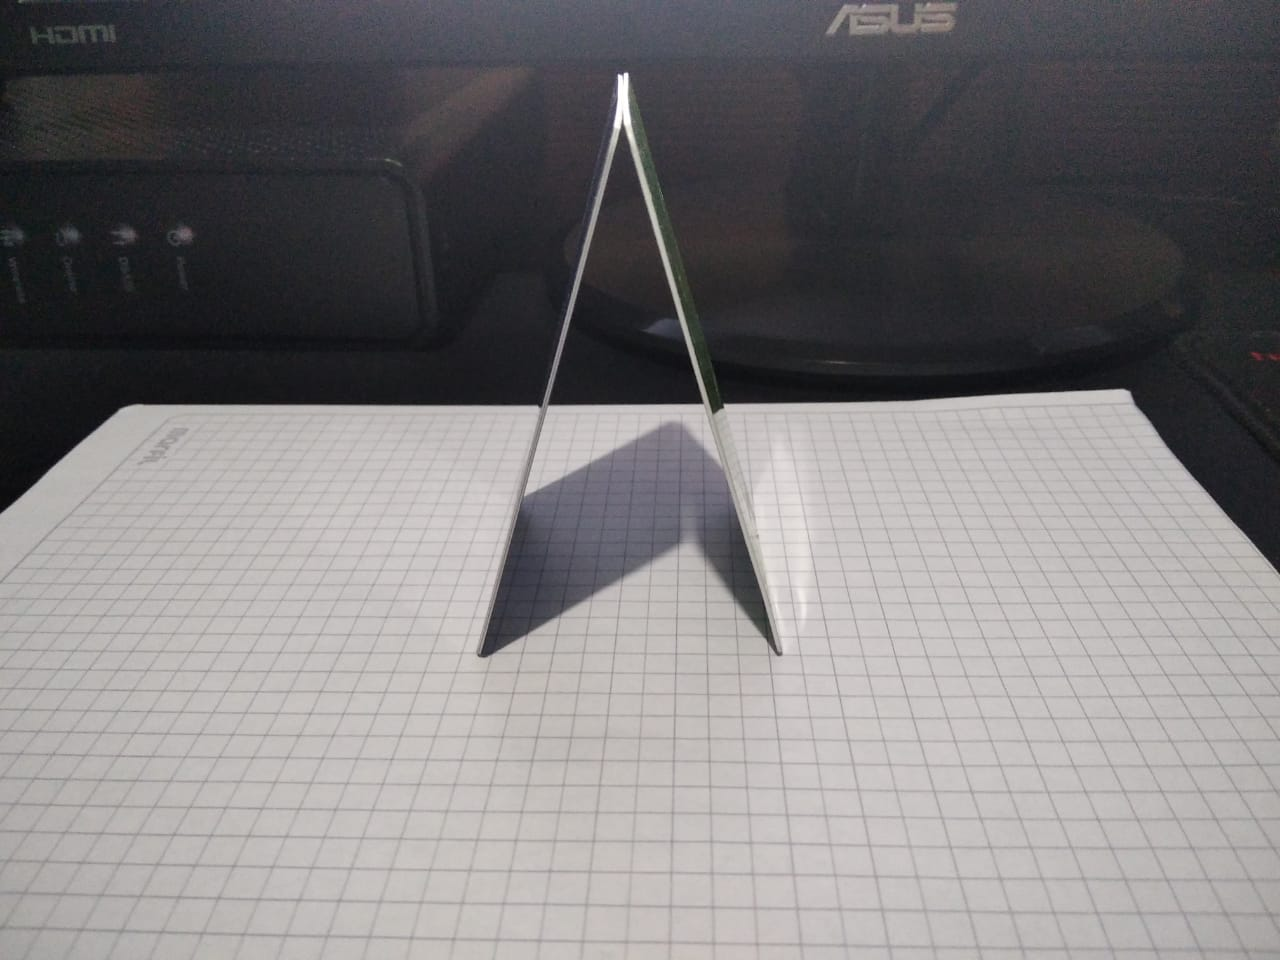
\includegraphics[width=4cm]{estado-final.jpeg}
\centering
\caption{Foto ejemplo del estado final}
\label{fig:estado-final}
\end{figure}

\newpage




\end{document}
